\documentclass[11pt,a4paper]{article}
\usepackage[utf8]{inputenc}
\usepackage[T1]{fontenc}
\usepackage[brazilian]{babel}
\usepackage{amsmath, amssymb}
\usepackage{booktabs}
\usepackage{longtable}
\usepackage{graphicx}
\usepackage{geometry}
\geometry{margin=2.5cm}

% gerado por scripts/gerar_analise.py — não editar à mão
\newcommand{\grauConfianca}{81,0\%}
\newcommand{\nJogosBacktest}{56}
\newcommand{\nDecididos}{42}
\newcommand{\nAcertos}{34}
\newcommand{\nEmpatesExcluidos}{14}
\newcommand{\favoritoTitulo}{Argentina}
\newcommand{\probFavorito}{17,5\%}
\newcommand{\probBrasil}{8,4\%}
\newcommand{\posBrasil}{3\textsuperscript{o}}
\newcommand{\dataAnalise}{2026-06-25}


\title{Previsor de Resultados da Copa do Mundo de 2026:\\
Metodologia, Verifica\c{c}\~ao Emp\'irica e Probabilidade de T\'itulo}
\author{richmo.media}
\date{\dataAnalise}

\begin{document}
\maketitle

\begin{abstract}
Este artigo descreve o m\'etodo usado para prever resultados da Copa de 2026 a
partir da forma recente das sele\c{c}\~oes, verifica-o empiricamente por uma
an\'alise regressiva (\emph{backtest}) sobre os jogos j\'a disputados e projeta
a probabilidade de cada sele\c{c}\~ao ser campe\~a por encadeamento das
probabilidades de vit\'oria no mata-mata.
\end{abstract}

\section{Introdu\c{c}\~ao}
O objetivo do previsor \'e gerar, para um bol\~ao, o palpite que maximiza os
pontos esperados. A metodologia combina a forma recente (janela de 90 dias),
um modelo de for\c{c}a ofensiva/defensiva e a distribui\c{c}\~ao de Poisson para
os gols.

\section{Metodologia}
\subsection{Coleta e janela de 90 dias}
Para cada partida a prever, consideram-se apenas os jogos das 48 sele\c{c}\~oes
nos \'ultimos 90 dias, capturando a forma recente.

\subsection{For\c{c}a ofensiva e defensiva (modelo circular)}
Cada sele\c{c}\~ao $i$ tem for\c{c}a de ataque $O_i$ e fragilidade defensiva
$D_i$. Sendo $\mu$ a m\'edia de gols por time por jogo, os gols esperados de $i$
contra $j$ s\~ao $\mu\,O_i\,D_j$. Como ataque depende da defesa do advers\'ario
e vice-versa, resolve-se o sistema por ponto fixo:
\begin{align}
O_i &\leftarrow \frac{\sum_{m} g^{\text{pro}}_{i,m}}
                     {\sum_{m} \mu\,D_{\text{adv}(i,m)}}, &
D_i &\leftarrow \frac{\sum_{m} g^{\text{contra}}_{i,m}}
                     {\sum_{m} \mu\,O_{\text{adv}(i,m)}},
\end{align}
iterando at\'e a converg\^encia. Uma regulariza\c{c}\~ao (encolhimento para
$O=D=1$) estabiliza estimativas de amostras pequenas.

\subsection{Gols esperados}
Com a for\c{c}a estimada, os gols esperados de mandante e visitante s\~ao
\begin{equation}
\lambda_{\text{casa}} = \mu\,O_{\text{casa}}\,D_{\text{fora}}, \qquad
\lambda_{\text{fora}} = \mu\,O_{\text{fora}}\,D_{\text{casa}},
\end{equation}
e a probabilidade de cada placar $(x,y)$ segue dois processos de Poisson
independentes: $P(x,y) = \mathrm{Pois}(x;\lambda_{\text{casa}})\,
\mathrm{Pois}(y;\lambda_{\text{fora}})$.

\subsection{Palpite \'otimo (resumo)}
O palpite recomendado \'e o placar que maximiza o valor esperado da fun\c{c}\~ao
de pontua\c{c}\~ao do bol\~ao sobre toda a matriz de placares. Esse passo
importa apenas para o placar exato (aposta/bol\~ao) e n\~ao para as an\'alises
de \emph{resultado} (vit\'oria/empate/derrota) deste artigo.

\section{Verifica\c{c}\~ao emp\'irica (\emph{backtest} walk-forward)}
Voltamos ao primeiro jogo da Copa e avan\c{c}amos jogo a jogo. Para cada partida
j\'a disputada, a for\c{c}a \'e recalculada usando \textbf{apenas} os dados
anteriores \`aquele jogo (sem vi\'es de futuro) e prev\^e-se o resultado de maior
probabilidade entre vit\'oria da casa, empate e vit\'oria de fora — somando as
regi\~oes da matriz de placares. Comparando com o resultado real, obtemos um
\textbf{grau de confian\c{c}a emp\'irico} (acerto do vencedor) de
\textbf{\grauConfianca} nos \nDecididos{} jogos decididos (\nAcertos{} acertos).

\paragraph{Por que excluir os empates.} Dos \nJogosBacktest{} jogos disputados,
\nEmpatesExcluidos{} terminaram empatados e foram exclu\'idos do c\'alculo da
confian\c{c}a. Ao tomar o resultado de \emph{maior probabilidade}, o m\'etodo
quase nunca aponta o empate — que exige duas sele\c{c}\~oes de baixa produ\c{c}\~ao
ofensiva \emph{e} for\c{c}as semelhantes — de modo que todo empate real viraria,
mecanicamente, um erro. Como o grau de confian\c{c}a serve para caucionar a
proje\c{c}\~ao de t\'itulo, que trata o mata-mata (onde n\~ao h\'a empates: a
decis\~ao vai aos p\^enaltis), a m\'etrica relevante \'e o acerto do
\emph{vencedor} nos jogos decididos. A tabela abaixo, ainda assim, lista
\emph{todos} os jogos, marcando os empates como erro para total transpar\^encia.

{\footnotesize% gerado por scripts/gerar_analise.py — não editar à mão
\begin{longtable}{llcccll c}
\toprule
Data & Jogo & P(C) & P(E) & P(F) & Prev. & Real & OK \\
\midrule
\endhead
2026-06-11 & México $\times$ África do Sul & 59,7\% & 30,4\% & 9,9\% & Casa & Casa & \checkmark \\
2026-06-12 & Coreia do Sul $\times$ República Tcheca & 57,1\% & 19,9\% & 23,0\% & Casa & Casa & \checkmark \\
2026-06-12 & Canadá $\times$ Bósnia e Herzegovina & 40,2\% & 34,3\% & 25,5\% & Casa & Empate & $\times$ \\
2026-06-13 & Estados Unidos $\times$ Paraguai & 22,1\% & 20,9\% & 57,0\% & Fora & Casa & $\times$ \\
2026-06-13 & Catar $\times$ Suíça & 12,9\% & 24,4\% & 62,7\% & Fora & Empate & $\times$ \\
2026-06-13 & Brasil $\times$ Marrocos & 30,1\% & 20,8\% & 49,1\% & Fora & Empate & $\times$ \\
2026-06-14 & Haiti $\times$ Escócia & 14,7\% & 20,7\% & 64,6\% & Fora & Fora & \checkmark \\
2026-06-14 & Austrália $\times$ Turquia & 35,0\% & 31,8\% & 33,2\% & Casa & Casa & \checkmark \\
2026-06-14 & Alemanha $\times$ Curaçao & 82,1\% & 10,0\% & 7,9\% & Casa & Casa & \checkmark \\
2026-06-14 & Holanda $\times$ Japão & 25,7\% & 35,2\% & 39,1\% & Fora & Empate & $\times$ \\
2026-06-14 & Costa do Marfim $\times$ Equador & 56,6\% & 25,3\% & 18,1\% & Casa & Casa & \checkmark \\
2026-06-15 & Suécia $\times$ Tunísia & 42,7\% & 25,5\% & 31,8\% & Casa & Casa & \checkmark \\
2026-06-15 & Espanha $\times$ Cabo Verde & 67,4\% & 18,1\% & 14,5\% & Casa & Empate & $\times$ \\
2026-06-15 & Bélgica $\times$ Egito & 54,1\% & 24,7\% & 21,2\% & Casa & Empate & $\times$ \\
2026-06-15 & Arábia Saudita $\times$ Uruguai & 15,6\% & 24,9\% & 59,4\% & Fora & Empate & $\times$ \\
2026-06-16 & Irã $\times$ Nova Zelândia & 68,9\% & 18,2\% & 12,9\% & Casa & Empate & $\times$ \\
2026-06-16 & França $\times$ Senegal & 54,9\% & 22,8\% & 22,3\% & Casa & Casa & \checkmark \\
2026-06-16 & Iraque $\times$ Noruega & 16,9\% & 27,9\% & 55,3\% & Fora & Fora & \checkmark \\
2026-06-17 & Argentina $\times$ Argélia & 20,9\% & 26,6\% & 52,5\% & Fora & Casa & $\times$ \\
2026-06-17 & Áustria $\times$ Jordânia & 84,2\% & 10,5\% & 5,4\% & Casa & Casa & \checkmark \\
2026-06-17 & Portugal $\times$ RD Congo & 51,0\% & 32,4\% & 16,6\% & Casa & Empate & $\times$ \\
2026-06-17 & Inglaterra $\times$ Croácia & 44,4\% & 29,5\% & 26,1\% & Casa & Casa & \checkmark \\
2026-06-17 & Gana $\times$ Panamá & 28,1\% & 18,8\% & 53,1\% & Fora & Casa & $\times$ \\
2026-06-18 & Uzbequistão $\times$ Colômbia & 26,7\% & 25,8\% & 47,5\% & Fora & Fora & \checkmark \\
2026-06-18 & República Tcheca $\times$ África do Sul & 40,7\% & 28,7\% & 30,6\% & Casa & Empate & $\times$ \\
2026-06-18 & Suíça $\times$ Bósnia e Herzegovina & 57,9\% & 25,1\% & 17,0\% & Casa & Casa & \checkmark \\
2026-06-18 & Canadá $\times$ Catar & 37,9\% & 36,1\% & 26,0\% & Casa & Casa & \checkmark \\
2026-06-19 & México $\times$ Coreia do Sul & 62,8\% & 23,3\% & 14,0\% & Casa & Casa & \checkmark \\
2026-06-19 & Estados Unidos $\times$ Austrália & 24,3\% & 22,5\% & 53,2\% & Fora & Casa & $\times$ \\
2026-06-19 & Escócia $\times$ Marrocos & 28,3\% & 28,6\% & 43,1\% & Fora & Fora & \checkmark \\
2026-06-20 & Brasil $\times$ Haiti & 71,2\% & 16,7\% & 12,1\% & Casa & Casa & \checkmark \\
2026-06-20 & Turquia $\times$ Paraguai & 38,5\% & 26,7\% & 34,8\% & Casa & Fora & $\times$ \\
2026-06-20 & Holanda $\times$ Suécia & 59,2\% & 17,6\% & 23,3\% & Casa & Casa & \checkmark \\
2026-06-20 & Alemanha $\times$ Costa do Marfim & 18,7\% & 21,4\% & 59,9\% & Fora & Casa & $\times$ \\
2026-06-21 & Equador $\times$ Curaçao & 82,7\% & 10,7\% & 6,6\% & Casa & Empate & $\times$ \\
2026-06-21 & Tunísia $\times$ Japão & 8,3\% & 23,3\% & 68,3\% & Fora & Fora & \checkmark \\
2026-06-21 & Espanha $\times$ Arábia Saudita & 56,4\% & 26,3\% & 17,3\% & Casa & Casa & \checkmark \\
2026-06-21 & Bélgica $\times$ Irã & 74,8\% & 15,0\% & 10,1\% & Casa & Empate & $\times$ \\
2026-06-21 & Uruguai $\times$ Cabo Verde & 48,5\% & 28,6\% & 22,9\% & Casa & Empate & $\times$ \\
2026-06-22 & Nova Zelândia $\times$ Egito & 8,7\% & 16,6\% & 74,7\% & Fora & Fora & \checkmark \\
2026-06-22 & Argentina $\times$ Áustria & 49,2\% & 26,7\% & 24,0\% & Casa & Casa & \checkmark \\
2026-06-22 & França $\times$ Iraque & 80,0\% & 12,5\% & 7,6\% & Casa & Casa & \checkmark \\
2026-06-23 & Noruega $\times$ Senegal & 54,0\% & 25,2\% & 20,7\% & Casa & Casa & \checkmark \\
2026-06-23 & Jordânia $\times$ Argélia & 5,1\% & 9,6\% & 85,3\% & Fora & Fora & \checkmark \\
2026-06-23 & Portugal $\times$ Uzbequistão & 59,7\% & 25,3\% & 15,1\% & Casa & Casa & \checkmark \\
2026-06-23 & Inglaterra $\times$ Gana & 62,1\% & 22,9\% & 15,0\% & Casa & Empate & $\times$ \\
2026-06-23 & Panamá $\times$ Croácia & 31,2\% & 19,3\% & 49,5\% & Fora & Fora & \checkmark \\
2026-06-24 & Colômbia $\times$ RD Congo & 47,2\% & 27,9\% & 24,9\% & Casa & Casa & \checkmark \\
2026-06-24 & Suíça $\times$ Canadá & 47,2\% & 22,9\% & 29,9\% & Casa & Casa & \checkmark \\
2026-06-24 & Bósnia e Herzegovina $\times$ Catar & 47,8\% & 31,9\% & 20,3\% & Casa & Casa & \checkmark \\
2026-06-24 & Marrocos $\times$ Haiti & 76,7\% & 16,3\% & 7,0\% & Casa & Casa & \checkmark \\
2026-06-24 & Escócia $\times$ Brasil & 30,5\% & 25,8\% & 43,7\% & Fora & Fora & \checkmark \\
2026-06-25 & República Tcheca $\times$ México & 6,4\% & 13,6\% & 80,0\% & Fora & Fora & \checkmark \\
2026-06-25 & África do Sul $\times$ Coreia do Sul & 19,6\% & 31,6\% & 48,8\% & Fora & Casa & $\times$ \\
2026-06-25 & Equador $\times$ Alemanha & 23,0\% & 26,0\% & 51,0\% & Fora & Casa & $\times$ \\
2026-06-25 & Curaçao $\times$ Costa do Marfim & 2,5\% & 5,7\% & 91,8\% & Fora & Fora & \checkmark \\
2026-06-25 & Tunísia $\times$ Holanda & 5,2\% & 12,7\% & 82,1\% & Fora & Fora & \checkmark \\
2026-06-25 & Japão $\times$ Suécia & 78,3\% & 12,5\% & 9,1\% & Casa & Empate & $\times$ \\
2026-06-26 & Turquia $\times$ Estados Unidos & 26,3\% & 22,9\% & 50,8\% & Fora & Casa & $\times$ \\
2026-06-26 & Paraguai $\times$ Austrália & 28,0\% & 25,3\% & 46,8\% & Fora & Empate & $\times$ \\
2026-06-26 & Noruega $\times$ França & 38,4\% & 23,8\% & 37,7\% & Casa & Fora & $\times$ \\
2026-06-26 & Senegal $\times$ Iraque & 59,0\% & 21,8\% & 19,2\% & Casa & Casa & \checkmark \\
2026-06-27 & Uruguai $\times$ Espanha & 20,6\% & 28,7\% & 50,7\% & Fora & Fora & \checkmark \\
2026-06-27 & Cabo Verde $\times$ Arábia Saudita & 54,0\% & 24,8\% & 21,2\% & Casa & Empate & $\times$ \\
2026-06-27 & Nova Zelândia $\times$ Bélgica & 6,5\% & 11,7\% & 81,8\% & Fora & Fora & \checkmark \\
2026-06-27 & Egito $\times$ Irã & 29,2\% & 35,3\% & 35,5\% & Fora & Empate & $\times$ \\
2026-06-27 & Panamá $\times$ Inglaterra & 17,5\% & 20,4\% & 62,1\% & Fora & Fora & \checkmark \\
2026-06-27 & Croácia $\times$ Gana & 32,0\% & 31,8\% & 36,2\% & Fora & Casa & $\times$ \\
2026-06-27 & Colômbia $\times$ Portugal & 21,3\% & 25,3\% & 53,4\% & Fora & Empate & $\times$ \\
2026-06-27 & RD Congo $\times$ Uzbequistão & 47,5\% & 32,9\% & 19,7\% & Casa & Casa & \checkmark \\
2026-06-28 & Jordânia $\times$ Argentina & 1,5\% & 4,4\% & 94,1\% & Fora & Fora & \checkmark \\
2026-06-28 & Argélia $\times$ Áustria & 25,8\% & 36,0\% & 38,2\% & Fora & Empate & $\times$ \\
\bottomrule
\end{longtable}
}

\section{Probabilidade de t\'itulo}
Como a fase de grupos ainda n\~ao terminou, os jogos faltantes s\~ao preenchidos
com o resultado previsto pelo m\'etodo, fixando os 32 confrontos das oitavas.
A partir da\'i, encadeamos as probabilidades: a chance de um time vencer um jogo
soma sobre os poss\'iveis advers\'arios, cada um ponderado pela sua probabilidade
de chegar \`aquele jogo (empate decidido nos p\^enaltis como moeda justa).
O produto ao longo das rodadas d\'a a probabilidade de t\'itulo. O favorito
segundo o m\'etodo \'e \textbf{\favoritoTitulo}. Estas proje\c{c}\~oes devem ser
lidas \`a luz do grau de confian\c{c}a emp\'irico (\grauConfianca).

\begin{figure}[h]
\centering
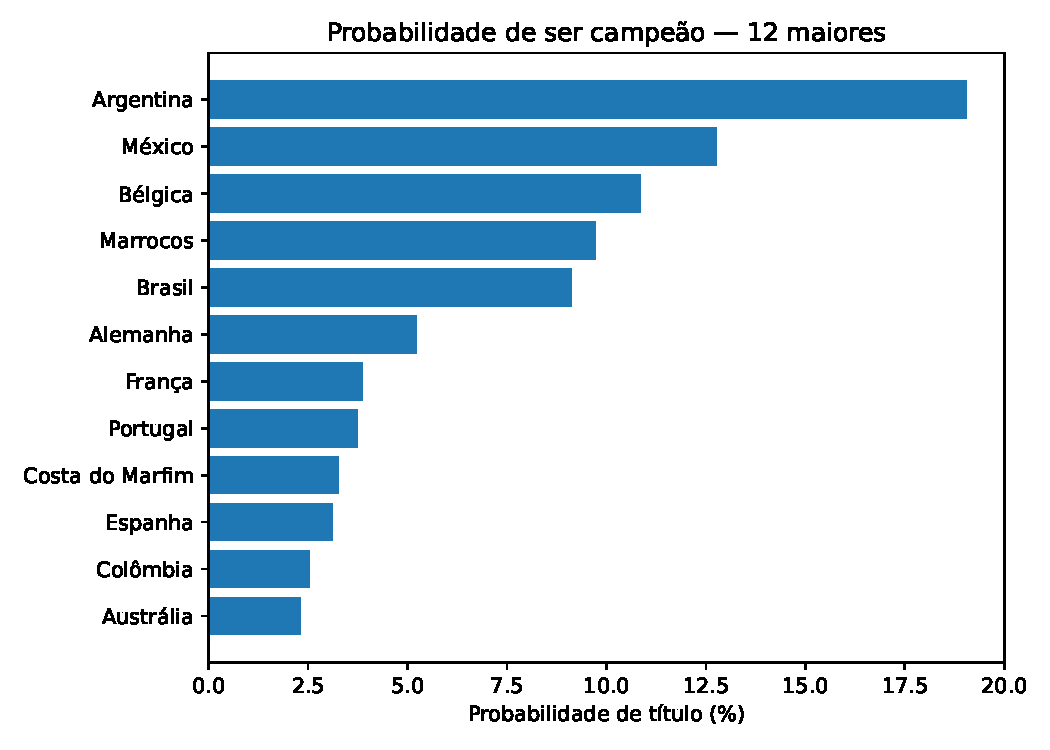
\includegraphics[width=0.8\textwidth]{figuras/titulo.pdf}
\caption{Probabilidade de t\'itulo das 12 sele\c{c}\~oes mais prov\'aveis.}
\end{figure}

{\footnotesize% gerado por scripts/gerar_analise.py — não editar à mão
\begin{longtable}{lccccc}
\toprule
Sele\c{c}\~ao & R32 & R16 & QF & SF & Campe\~ao \\
\midrule
\endhead
Argentina & 78,9\% & 60,9\% & 44,0\% & 30,0\% & 19,1\% \\
México & 69,5\% & 50,4\% & 31,5\% & 21,0\% & 12,8\% \\
Bélgica & 77,4\% & 55,9\% & 36,0\% & 19,9\% & 10,9\% \\
Marrocos & 75,2\% & 57,2\% & 35,1\% & 18,2\% & 9,7\% \\
Brasil & 69,2\% & 45,3\% & 25,5\% & 16,0\% & 9,1\% \\
Alemanha & 67,5\% & 41,4\% & 23,3\% & 10,8\% & 5,2\% \\
França & 85,1\% & 42,2\% & 21,5\% & 8,9\% & 3,9\% \\
Portugal & 71,7\% & 39,3\% & 19,0\% & 8,6\% & 3,7\% \\
Costa do Marfim & 61,5\% & 28,1\% & 13,3\% & 6,8\% & 3,3\% \\
Espanha & 59,9\% & 33,1\% & 15,9\% & 7,2\% & 3,1\% \\
Colômbia & 66,3\% & 33,7\% & 13,6\% & 6,3\% & 2,5\% \\
Austrália & 52,9\% & 29,7\% & 12,1\% & 5,6\% & 2,3\% \\
Inglaterra & 68,9\% & 26,7\% & 11,5\% & 5,3\% & 2,3\% \\
Estados Unidos & 79,4\% & 30,6\% & 15,3\% & 6,0\% & 2,2\% \\
Suíça & 63,0\% & 20,2\% & 10,2\% & 4,4\% & 1,6\% \\
Egito & 47,1\% & 25,0\% & 9,5\% & 4,1\% & 1,6\% \\
Equador & 30,5\% & 16,2\% & 6,5\% & 2,8\% & 1,1\% \\
Japão & 30,8\% & 14,4\% & 5,8\% & 2,4\% & 1,0\% \\
Áustria & 40,1\% & 17,8\% & 6,5\% & 2,3\% & 0,7\% \\
Paraguai & 32,5\% & 14,0\% & 5,7\% & 1,9\% & 0,7\% \\
Canadá & 59,8\% & 18,9\% & 6,4\% & 1,9\% & 0,6\% \\
Noruega & 38,5\% & 12,2\% & 4,4\% & 1,6\% & 0,6\% \\
Cabo Verde & 21,1\% & 9,8\% & 4,2\% & 1,5\% & 0,5\% \\
Holanda & 24,8\% & 14,0\% & 4,8\% & 1,4\% & 0,4\% \\
Senegal & 22,6\% & 9,9\% & 3,9\% & 1,2\% & 0,3\% \\
Argélia & 37,0\% & 9,1\% & 3,5\% & 1,1\% & 0,3\% \\
Gana & 33,7\% & 11,6\% & 2,9\% & 0,9\% & 0,2\% \\
África do Sul & 40,2\% & 10,0\% & 2,6\% & 0,6\% & 0,2\% \\
Croácia & 28,3\% & 9,8\% & 2,5\% & 0,6\% & 0,1\% \\
RD Congo & 31,1\% & 6,7\% & 1,6\% & 0,4\% & 0,1\% \\
Bósnia e Herzegovina & 20,6\% & 3,5\% & 0,9\% & 0,2\% & 0,0\% \\
Suécia & 14,9\% & 2,4\% & 0,5\% & 0,1\% & 0,0\% \\
\bottomrule
\end{longtable}
}

\section{Reprodutibilidade}
Todas as tabelas e a figura s\~ao geradas por
\texttt{scripts/gerar\_analise.py}, que consome os resultados reais da API e
reexecuta os c\'alculos. Conforme novos jogos ocorrem (fim da fase de grupos,
mata-mata), basta reexecutar o script para atualizar o artigo.

\end{document}
